%%%%%%%%%%%%%%%%%%%% author.tex %%%%%%%%%%%%%%%%%%%%%%%%%%%%%%%%%%%
%
% sample root file for your "contribution" to a contributed volume
%
% Use this file as a template for your own input.
%
%%%%%%%%%%%%%%%% Springer %%%%%%%%%%%%%%%%%%%%%%%%%%%%%%%%%%


% RECOMMENDED %%%%%%%%%%%%%%%%%%%%%%%%%%%%%%%%%%%%%%%%%%%%%%%%%%%
\documentclass[graybox]{svmult}

% choose options for [] as required from the list
% in the Reference Guide

\usepackage{bibentry}
\usepackage{type1cm}        % activate if the above 3 fonts are
                            % not available on your system
%
\usepackage{makeidx}         % allows index generation
\usepackage{graphicx}        % standard LaTeX graphics tool
                             % when including figure files
\usepackage{multicol}        % used for the two-column index
\usepackage[bottom]{footmisc}% places footnotes at page bottom

\usepackage{newtxtext}       %
\usepackage{newtxmath}       % selects Times Roman as basic font
\usepackage{dirtytalk} \newcommand{\mysay}[1]{\say{\textit{#1}}}
\usepackage{enumerate}
\usepackage[unicode,colorlinks=true,breaklinks,allcolors=black]{hyperref}
\usepackage{cleveref}
\usepackage{ltablex}
\usepackage{booktabs}
\usepackage{makecell}
\usepackage{doi}
\usepackage{enumitem}

% Probably should be swapped for JPEGs!
\usepackage{pgfplots}
\usepgfplotslibrary{statistics}
\usetikzlibrary{pgfplots.statistics} % LATEX and plain TEX
\usetikzlibrary[pgfplots.statistics] % ConTEXt

%\nobibliography
\usepackage{fixme}

\nobibliography*


% see the list of further useful packages
% in the Reference Guide

\makeindex             % used for the subject index
                       % please use the style svind.ist with
                       % your makeindex program

%%%%%%%%%%%%%%%%%%%%%%%%%%%%%%%%%%%%%%%%%%%%%%%%%%%%%%%%%%%%%%%%%%%%%%%%%%%%%%%%%%%%%%%%%



\begin{document}

\title*{Sprawozdanie z Milestone'u \#1 Grupy M2}
\author{Marcel Jerzyk, Jakub Litkowski, Jakub Szańca}
\institute{
Marcel Jerzyk \at Wroclaw University of Science and Technology, Poland, \email{244979@student.pwr.edu.pl}
\and Jakub Litkowski \at Wroclaw University of Science and Technology, Poland, \email{242353@student.pwr.edu.pl}
\and Jakub Szańca \at Wroclaw University of Science and Technology, Poland, \email{242519@student.pwr.edu.pl}
}

\maketitle



\newpage

\section{Performance Test}

Uruchomienie programu przy pomocy komendy z \textit{README.md} ,,\textit{mvn exec:java}'' trwało:



\begin{table}[!h]
\centering
        
\begin{tabular}{|p{0.33\textwidth}|p{0.33\textwidth}|p{0.33\textwidth}|}
\hline 
 \begin{center}
\textbf{Komputer}
\end{center}
 & \begin{center}
\textbf{Próba}
\end{center}
 & \begin{center}
\textbf{Czas}
\end{center}
 \\
\hline 
 \multirow{$\displaystyle k_{1}$} & $\displaystyle 1$ & 13:52 \\
\cline{2-3} 
   & $\displaystyle 2$ & 13:42 \\
\cline{2-3} 
   & $\displaystyle 3$ & 13:37 \\
\hline 
 \multirow{$\displaystyle k_{2}$} & $\displaystyle 1$ & 24:47 \\
\cline{2-3} 
   & $\displaystyle 2$ & 24:51 \\
\cline{2-3} 
   & $\displaystyle 3$ & 25:02 \\
\hline 
 \multirow{$\displaystyle k_{2}$} & $\displaystyle 1$ & 56:28 \\
\cline{2-3} 
   & $\displaystyle 2$ & --- \\
\cline{2-3} 
   & $\displaystyle 3$ & --- \\
 \hline
\end{tabular}
        
\end{table}

Przy czym konfiguracja komputerów $k_{1}, k_{2}, k_{3}$ jest następująca:

\begin{table}[!h]
\centering
        
\begin{tabular}{|p{0.20\textwidth}|p{0.20\textwidth}|p{0.20\textwidth}|p{0.20\textwidth}|p{0.20\textwidth}|}
\hline 
 \begin{center}
\textbf{Komputer}
\end{center}
 & \begin{center}
\textbf{CPU}
\end{center}
 & \begin{center}
\textbf{GPU}
\end{center}
 & \begin{center}
\textbf{OS}
\end{center}
 & \begin{center}
\textbf{RAM}
\end{center}
 \\
\hline 
 $\displaystyle k_{1}$ & Ryzen 3600 & RTX 2060 2GB & Windows 10 & 32GB @ 1600MHz \\
\hline 
 $\displaystyle k_{2}$ & Intel Core i7  6820HQ & Intel HD Graphics 530  & Windows 10 & 16GB @ 1600 MHz \\
\hline 
 $\displaystyle k_{3}$ &Intel Core i5-7200U  &Intel HD Graphics 620  & Windows 10 & 12GB @ 2133MHz  \\
 \hline
\end{tabular}
        
\end{table}

Otrzymane wyniki w przypadku z każdego testu dla komputera $k_{1}$ były reprodukowalne (identyczne przy każdej próbie).

\begin{frame}{}
\hbox{\hspace{-5.0em} 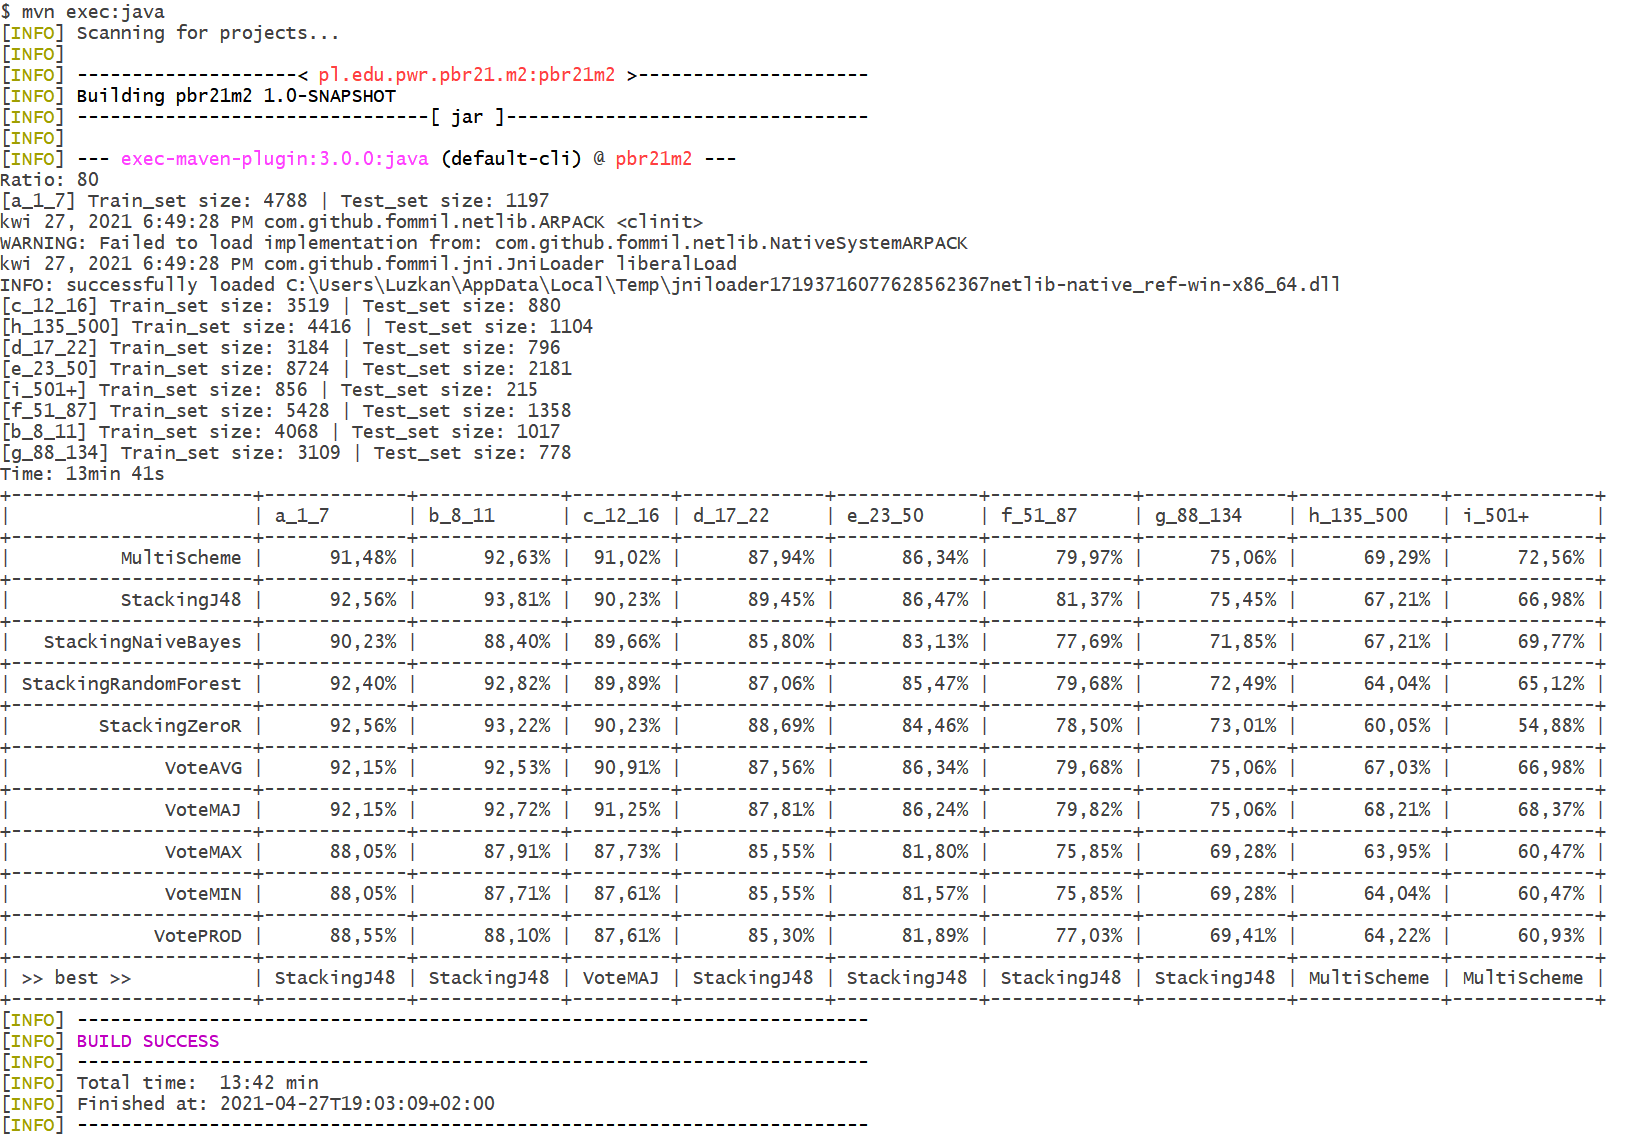
\includegraphics[scale=0.27]{img/results.png}}
\end{frame}



\section{Uwagi}

\subsection{\textit{README.md}}

Plik \textit{README.md} ma bardzo lakoniczny opis, który ujmuje tylko samą metodę aplikacji. Brakuje w nim informacji na temat tego, co się dokładnie dzieje po uruchomieniu danej komendy i w jakim celu się ją wykonuje. Brakuje informacji na temat rezultatu otrzymanych danych oraz ich definicji, aby móc zrozumieć istotę programu. Brak informacji o badanych meta klasyfikatorach. Brak zrzutu ekranu z przykładowych wyników.

Technicznie - brakuje w nim informacji na jakiej wersji \emph{Javy} można uruchomić program, bądź na jakiej był tworzony, a więc na jakiej powinien być testowany. Nie ma informacji na temat użytych bibliotek i ich wersji.

\subsection{Kod}

Kod aplikacji jest zrozumiały oraz dobrze podzielony na pakiety.

\subsection{Report}

Prezentujemy zaimportowane dane z wygenerowanego raportu w programie Excel. \\

\begin{frame}{}
\hbox{\hspace{-5.0em} 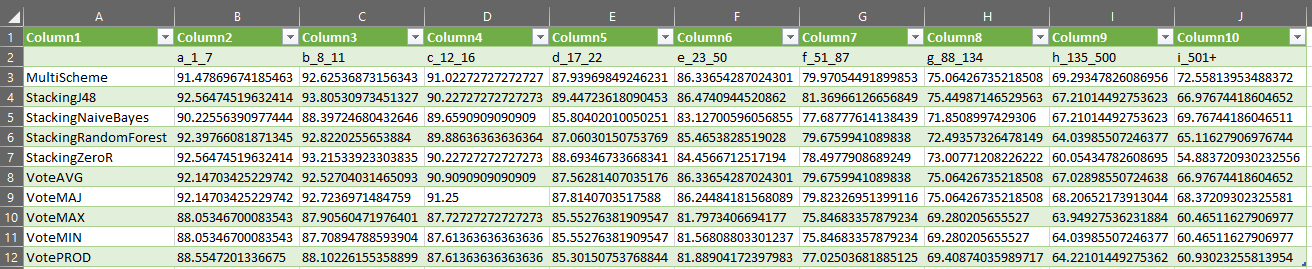
\includegraphics[scale=0.45]{img/results_loaded.png}}
\end{frame}
%%%%%%%%%%%%%%%%%%%%%%%%% referenc.tex %%%%%%%%%%%%%%%%%%%%%%%%%%%%%%
% sample references
% %
% Use this file as a template for your own input.
%
%%%%%%%%%%%%%%%%%%%%%%%% Springer-Verlag %%%%%%%%%%%%%%%%%%%%%%%%%%
%
% BibTeX users please use
% \bibliographystyle{}
% \bibliography{}
%
\biblstarthook{References may be \textit{cited} in the text either by number (preferred) or by author/year.\footnote{Make sure that all references from the list are cited in the text. Those not cited should be moved to a separate \textit{Further Reading} section or chapter.} If the citatiion in the text is numbered, the reference list should be arranged in ascending order. If the citation in the text is author/year, the reference list should be \textit{sorted} alphabetically and if there are several works by the same author, the following order should be used:
\begin{enumerate}
\item all works by the author alone, ordered chronologically by year of publication
\item all works by the author with a coauthor, ordered alphabetically by coauthor
\item all works by the author with several coauthors, ordered chronologically by year of publication.
\end{enumerate}
The \textit{styling} of references\footnote{Always use the standard abbreviation of a journal's name according to the ISSN \textit{List of Title Word Abbreviations}, see \url{http://www.issn.org/en/node/344}} depends on the subject of your book:
\begin{itemize}
\item The \textit{two} recommended styles for references in books on \textit{mathematical, physical, statistical and computer sciences} are depicted in ~\cite{science-contrib, science-online, science-mono, science-journal, science-DOI} and ~\cite{phys-online, phys-mono, phys-journal, phys-DOI, phys-contrib}.
\item Examples of the most commonly used reference style in books on \textit{Psychology, Social Sciences} are~\cite{psysoc-mono, psysoc-online,psysoc-journal, psysoc-contrib, psysoc-DOI}.
\item Examples for references in books on \textit{Humanities, Linguistics, Philosophy} are~\cite{humlinphil-journal, humlinphil-contrib, humlinphil-mono, humlinphil-online, humlinphil-DOI}.
\item Examples of the basic Springer Nature style used in publications on a wide range of subjects such as \textit{Computer Science, Economics, Engineering, Geosciences, Life Sciences, Medicine, Biomedicine} are ~\cite{basic-contrib, basic-online, basic-journal, basic-DOI, basic-mono}. 
\end{itemize}
}

\begin{thebibliography}{99.}%
% and use \bibitem to create references.
%
% Use the following syntax and markup for your references if 
% the subject of your book is from the field 
% "Mathematics, Physics, Statistics, Computer Science"
%
% Contribution 
\bibitem{science-contrib} Broy, M.: Software engineering --- from auxiliary to key technologies. In: Broy, M., Dener, E. (eds.) Software Pioneers, pp. 10-13. Springer, Heidelberg (2002)
%
% Online Document
\bibitem{science-online} Dod, J.: Effective substances. In: The Dictionary of Substances and Their Effects. Royal Society of Chemistry (1999) Available via DIALOG. \\
\url{http://www.rsc.org/dose/title of subordinate document. Cited 15 Jan 1999}
%
% Monograph
\bibitem{science-mono} Geddes, K.O., Czapor, S.R., Labahn, G.: Algorithms for Computer Algebra. Kluwer, Boston (1992) 
%
% Journal article
\bibitem{science-journal} Hamburger, C.: Quasimonotonicity, regularity and duality for nonlinear systems of partial differential equations. Ann. Mat. Pura. Appl. \textbf{169}, 321--354 (1995)
%
% Journal article by DOI
\bibitem{science-DOI} Slifka, M.K., Whitton, J.L.: Clinical implications of dysregulated cytokine production. J. Mol. Med. (2000) doi: 10.1007/s001090000086 
%
\bigskip

% Use the following (APS) syntax and markup for your references if 
% the subject of your book is from the field 
% "Mathematics, Physics, Statistics, Computer Science"
%
% Online Document
\bibitem{phys-online} J. Dod, in \textit{The Dictionary of Substances and Their Effects}, Royal Society of Chemistry. (Available via DIALOG, 1999), 
\url{http://www.rsc.org/dose/title of subordinate document. Cited 15 Jan 1999}
%
% Monograph
\bibitem{phys-mono} H. Ibach, H. L\"uth, \textit{Solid-State Physics}, 2nd edn. (Springer, New York, 1996), pp. 45-56 
%
% Journal article
\bibitem{phys-journal} S. Preuss, A. Demchuk Jr., M. Stuke, Appl. Phys. A \textbf{61}
%
% Journal article by DOI
\bibitem{phys-DOI} M.K. Slifka, J.L. Whitton, J. Mol. Med., doi: 10.1007/s001090000086
%
% Contribution 
\bibitem{phys-contrib} S.E. Smith, in \textit{Neuromuscular Junction}, ed. by E. Zaimis. Handbook of Experimental Pharmacology, vol 42 (Springer, Heidelberg, 1976), p. 593
%
\bigskip
%
% Use the following syntax and markup for your references if 
% the subject of your book is from the field 
% "Psychology, Social Sciences"
%
%
% Monograph
\bibitem{psysoc-mono} Calfee, R.~C., \& Valencia, R.~R. (1991). \textit{APA guide to preparing manuscripts for journal publication.} Washington, DC: American Psychological Association.
%
% Online Document
\bibitem{psysoc-online} Dod, J. (1999). Effective substances. In: The dictionary of substances and their effects. Royal Society of Chemistry. Available via DIALOG. \\
\url{http://www.rsc.org/dose/Effective substances.} Cited 15 Jan 1999.
%
% Journal article
\bibitem{psysoc-journal} Harris, M., Karper, E., Stacks, G., Hoffman, D., DeNiro, R., Cruz, P., et al. (2001). Writing labs and the Hollywood connection. \textit{J Film} Writing, 44(3), 213--245.
%
% Contribution 
\bibitem{psysoc-contrib} O'Neil, J.~M., \& Egan, J. (1992). Men's and women's gender role journeys: Metaphor for healing, transition, and transformation. In B.~R. Wainrig (Ed.), \textit{Gender issues across the life cycle} (pp. 107--123). New York: Springer.
%
% Journal article by DOI
\bibitem{psysoc-DOI}Kreger, M., Brindis, C.D., Manuel, D.M., Sassoubre, L. (2007). Lessons learned in systems change initiatives: benchmarks and indicators. \textit{American Journal of Community Psychology}, doi: 10.1007/s10464-007-9108-14.
%
%
% Use the following syntax and markup for your references if 
% the subject of your book is from the field 
% "Humanities, Linguistics, Philosophy"
%
\bigskip
%
% Journal article
\bibitem{humlinphil-journal} Alber John, Daniel C. O'Connell, and Sabine Kowal. 2002. Personal perspective in TV interviews. \textit{Pragmatics} 12:257--271
%
% Contribution 
\bibitem{humlinphil-contrib} Cameron, Deborah. 1997. Theoretical debates in feminist linguistics: Questions of sex and gender. In \textit{Gender and discourse}, ed. Ruth Wodak, 99--119. London: Sage Publications.
%
% Monograph
\bibitem{humlinphil-mono} Cameron, Deborah. 1985. \textit{Feminism and linguistic theory.} New York: St. Martin's Press.
%
% Online Document
\bibitem{humlinphil-online} Dod, Jake. 1999. Effective substances. In: The dictionary of substances and their effects. Royal Society of Chemistry. Available via DIALOG. \\
http://www.rsc.org/dose/title of subordinate document. Cited 15 Jan 1999
%
% Journal article by DOI
\bibitem{humlinphil-DOI} Suleiman, Camelia, Daniel C. O'Connell, and Sabine Kowal. 2002. `If you and I, if we, in this later day, lose that sacred fire...': Perspective in political interviews. \textit{Journal of Psycholinguistic Research}. doi: 10.1023/A:1015592129296.
%
%
%
\bigskip
%
%
% Use the following syntax and markup for your references if 
% the subject of your book is from the field 
% "Computer Science, Economics, Engineering, Geosciences, Life Sciences"
%
%
% Contribution 
\bibitem{basic-contrib} Brown B, Aaron M (2001) The politics of nature. In: Smith J (ed) The rise of modern genomics, 3rd edn. Wiley, New York 
%
% Online Document
\bibitem{basic-online} Dod J (1999) Effective Substances. In: The dictionary of substances and their effects. Royal Society of Chemistry. Available via DIALOG. \\
\url{http://www.rsc.org/dose/title of subordinate document. Cited 15 Jan 1999}
%
% Journal article by DOI
\bibitem{basic-DOI} Slifka MK, Whitton JL (2000) Clinical implications of dysregulated cytokine production. J Mol Med, doi: 10.1007/s001090000086
%
% Journal article
\bibitem{basic-journal} Smith J, Jones M Jr, Houghton L et al (1999) Future of health insurance. N Engl J Med 965:325--329
%
% Monograph
\bibitem{basic-mono} South J, Blass B (2001) The future of modern genomics. Blackwell, London 
%
\end{thebibliography}

\end{document}
